\begin{figure}[htb]
    \centering
    \begin{subfigure}[b]{0.45\textwidth}
        \centering
        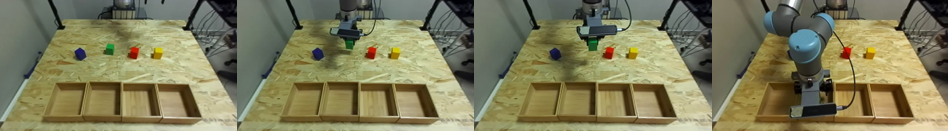
\includegraphics[width=\textwidth]{Figures/images/dataset_real_robot/frontal_camera.png}
        \caption{Frames of pick-place task from frontal camera}
        \label{fig:frontal_camera}
    \end{subfigure}
    \hspace{5px}
    \begin{subfigure}[b]{0.45\textwidth}
        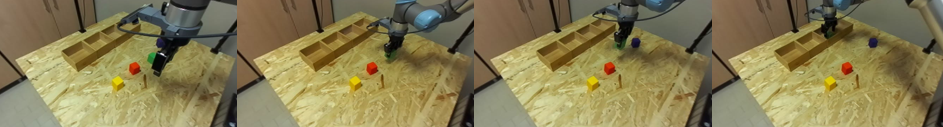
\includegraphics[width=\textwidth]{Figures/images/dataset_real_robot/lateral_left.png}
        \caption{Frames of pick-place task from lateral left camera}
        \label{fig:lateral_left}
    \end{subfigure}
    \vfill
    \begin{subfigure}[b]{0.45\textwidth}
        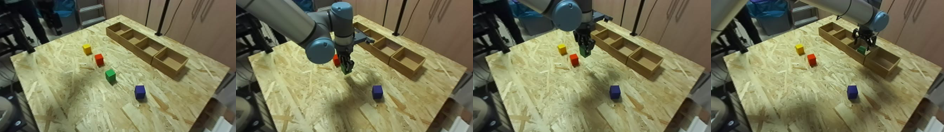
\includegraphics[width=\textwidth]{Figures/images/dataset_real_robot/lateral_right.png}
        \caption{Frames of pick-place task from lateral right camera}
        \label{fig:lateral_right}
    \end{subfigure}
    \hspace{5px}
    \begin{subfigure}[b]{0.45\textwidth}
        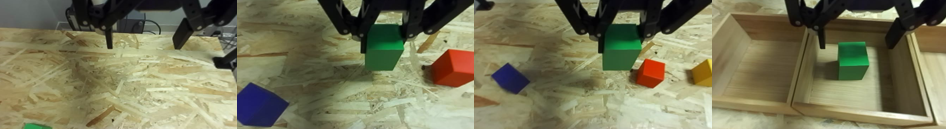
\includegraphics[width=\textwidth]{Figures/images/dataset_real_robot/gripper_camera.png}
        \caption{Frames of pick-place task from gripper camera}
        \label{fig:gripper_camera}
    \end{subfigure}
    \caption{Frames of pick-place task from different cameras}
    \label{fig:real_dataset}
\end{figure}

